\documentclass[11pt]{article}
\usepackage[T1]{fontenc}
\usepackage{lmodern}
\usepackage[utf8]{inputenc}
\usepackage[margin=1in]{geometry}
\usepackage{amsmath,amssymb,amsthm}
\usepackage{graphicx,booktabs,xcolor}
\usepackage{listings}
\usepackage[hidelinks]{hyperref}
\lstset{basicstyle=\ttfamily\scriptsize,breaklines=true,columns=fullflexible,frame=single,framerule=0.3pt,rulecolor=\color{gray}}
\lstset{literate={²}{{$^2$}}1 {³}{{$^3$}}1 {·}{{$\cdot$}}1 {Γ}{{$\Gamma$}}1 {ν}{{$\nu$}}1 {π}{{$\pi$}}1 {ε}{{$\varepsilon$}}1 {₀}{{$_0$}}1 {₁}{{$_1$}}1 {₂}{{$_2$}}1 {ₖ}{{$_k$}}1 {ℂ}{{$\mathbb{C}$}}1 {ℝ}{{$\mathbb{R}$}}1 {←}{{$\leftarrow$}}1 {↔}{{$\leftrightarrow$}}1 {−}{{-}}1 {≠}{{$\neq$}}1 {≤}{{$\le$}}1 {⟨}{{$\langle$}}1 {⟩}{{$\rangle$}}1 {§}{{\S}}1 {½}{{$\frac12$}}1 {⁴}{{$^4$}}1 {⁵}{{$^5$}}1 {⁷}{{$^7$}}1 {⁸}{{$^8$}}1 {⁺}{{$^+$}}1 {⁻}{{$^-$}}1}
\newtheorem{theorem}{Theorem}
\newtheorem{proposition}[theorem]{Proposition}
\newtheorem{corollary}[theorem]{Corollary}
\theoremstyle{definition}
\newtheorem{definition}[theorem]{Definition}
\newcommand{\grade}[1]{\textsf{\small[#1]}}
\newcommand{\Tr}{\operatorname{Tr}}
\title{Matter, Then On Down\\[4pt]\large One coordinate from bulk matter to the nucleus}
\author{Jeromie Beasley}
\date{3 November 2026 \quad Draft v3}
\newcommand{\LEANSTATUS}{\emph{Status.} All twelve compile with no \texttt{sorry}, and every module is replayed by Lean's independent kernel checker. The axiom audit finds only \texttt{propext}, \texttt{Classical.choice} and \texttt{Quot.sound}, the three every Mathlib proof may use. A deliberately false companion, that the small-$s$ form $2s/S_{\mathrm{next}}$ is the exact rim distance, is rejected, as are the repository's fifteen other false controls. Checked by GitHub Actions, run 41729732315, commit \texttt{0e5792a} (152 theorems across the repository).}
\begin{document}
\maketitle

\noindent\emph{Prepared with AI assistance (Claude, Anthropic): the ideas and research direction are the author's; the computation, drafting and checking were done with AI tools. This draft was assembled from the author's published papers for his review.}

\begin{abstract}
Matter has no absolute size. The one place scale returns is a logarithmic boundary count whose coefficient is fixed by the central charge, $A=2c/\pi^2$ for an interval. This paper follows that boundary downward. At every scale the same function, $\Gamma=(z-1)/(z+1)=\tanh(\tfrac12\ln z)$, reads a ratio: occupation odds at a cut of bulk matter, successive removal energies of an atom, separation energies of a nucleus, and the complex odds of opened, non-Hermitian matter. The boundary census is the gauge without its sign; the signed offset $\tau=\log\det(I-C)-\log\det C$ is its clock face, and it moves only as fast as the coupling energy across the cut allows. The thermal entanglement ladder of the Ising chain is a peel ladder with one constant step. Helium's two thresholds give $\Gamma_0=0.377575$. The unbound nuclei ${}^5$He, ${}^5$Li and ${}^8$Be sit outside the disk at $|\Gamma|=1.074$, $1.220$, $1.025$, recomputed here from NUBASE2020, and their rapidity has turned half a revolution. Opened matter leaves the disk before its critical point; on the PT-symmetric chain the exit line is $E(0)E(\pi)=u^2$, equivalently a band-averaged Petermann factor of exactly 2, and the conditions under which that holds are stated with their counterexamples. Every claim carries a grade and every number a script. Appendix A proves every result the argument uses, including those imported from the author's earlier papers; Appendix B prints the Lean file that machine-checks the algebraic core; Appendix C prints every script, figure scripts included, with its output.
\end{abstract}

\paragraph{Grades.} \grade{T} proved here or in the cited paper of the author; \grade{V} verified numerically with stated controls; \grade{R} a reproduction of a known result in this coordinate; \grade{C} conjecture; \grade{H} a reading. \grade{lit} marks comparison with other people's published data.

\section{Matter has no absolute size}
Every instrument needs a zero and a span. In the operator framework of \emph{Matter at a Scale} (v5) and \emph{Foundational Operator Field Theory}, the zero is free and so is the span: difference observables are unchanged by $K\mapsto K+cI$, and spectral projectors, principal angles and the infrared boundary census are unchanged by $K\mapsto cK$ with $c>0$ \grade{T}. Only ratios are observable.

The single failure is ultraviolet. For a region $A$ with $|\partial A|$ boundary points in a substrate of correlation length $\xi$ and central charge $c$, the number $N$ of eigenvalues of the restricted correlation matrix in $[\varepsilon,1-\varepsilon]$ grows as
\begin{equation}
N=|\partial A|\,\frac{c}{\pi^2}\,\log\frac{\xi}{a}\,\log\frac1\varepsilon+\dots
\label{eq:census}
\end{equation}
so a two-endpoint interval carries $A=2c/\pi^2$ \grade{T}. The coefficient was measured at $c=1$ as $0.202692$ against $2/\pi^2=0.202642$, and at $c=\tfrac12$ (the transverse-field Ising chain) as $0.103689$, bracketing $1/\pi^2$ from both sides and $41.8$ times closer to it than to the $c=1$ value \grade{V}. \emph{The Angle Between the Rails} derives the same coefficient from the spacing $\Delta=4\pi K(\tilde u)/K'(\tilde u)$ of the entanglement ladder, $N=4\Lambda/\Delta$ for two cuts \grade{T}. A rescaling of the substrate is registered only as a running, never as a power.

The physical reading of \emph{Matter at a Scale} is the starting point of everything below: matter is a gap wearing a boundary. A gapped substrate keeps a finite, area-law census; gas, the gapless phase, floods it.

\section{The boundary keeps a ledger}
\subsection{Census, offset and one chart}
Let $C$ be the one-body correlation matrix of a region, with eigenvalues $\nu\in(0,1)$. Each level has odds $z=(1-\nu)/\nu$ and a rapidity $\varepsilon=\ln z$. Write $\Gamma=(z-1)/(z+1)$.

\begin{proposition}[the bridge] \label{prop:bridge}
$\Gamma=\tanh(\varepsilon/2)=1-2\nu$, and the window $\nu\in[\delta,1-\delta]$ is the disk $|\Gamma|\le1-2\delta$. The binary entropy integrated over the rapidity is $\int_{-\infty}^{\infty}H(\nu(\varepsilon))\,d\varepsilon=\pi^2/3$. \grade{T}
\end{proposition}
\begin{proof}
With $z=(1-\nu)/\nu$: $z-1=(1-2\nu)/\nu$ and $z+1=1/\nu$, so $\Gamma=1-2\nu$. Also $(e^\varepsilon-1)/(e^\varepsilon+1)=\tanh(\varepsilon/2)$. The window statement is $|1-2\nu|\le1-2\delta$. For the integral, $\nu=1/(1+e^\varepsilon)$ and $d\nu=-\nu(1-\nu)\,d\varepsilon$, so $\int H\,d\varepsilon=\int_0^1 H(\nu)/(\nu(1-\nu))\,d\nu=2\int_0^1(-\ln\nu)/(1-\nu)\,d\nu=2\zeta(2)=\pi^2/3$.
\end{proof}
Checked to $1.1\times10^{-16}$ and $6.7\times10^{-15}$ (script \texttt{s01}). The identity $1-2\nu=\tanh(\varepsilon/2)$ is standard in entanglement-spectrum work; the reading is the author's. \emph{The Offset Speed Limit} (Appendix B) names the same function four ways at once: the Smith-chart reflection $(z-1)/(z+1)$, the two-level Gibbs population gap $\tanh(\beta\Delta/2)$, the asymmetry $1-2\nu$ of an occupation against its log-odds, and the peel coordinate of VOTKP.

Summed over the levels of the region, the rapidity is the author's signed offset,
\begin{equation}
\tau=\sum_\nu \varepsilon_\nu=\Tr[\log(I-C)-\log C]=\log\frac{\det(I-C)}{\det C}=\log\frac{P(N_A=0)}{P(N_A=|A|)},
\end{equation}
the log-odds of the region being empty against full (\emph{The Offset Belongs to the Boundary}, v31, Theorem 2) \grade{T}. The census counts levels inside a window of $\nu(1-\nu)$, and $\nu(1-\nu)=(1-\Gamma^2)/4$ is blind to the sign of $\Gamma$. In the author's words: ``The offset is the clock face; the census is the gauge without its sign.'' The census of $\mathrm{diag}(0.2,0.8)$ and of $\mathrm{diag}(0.2,0.2)$ is the same $0.16I$; their offsets are $0$ and $\log16$.

\subsection{The weight between and the speed of the record}
Split the space into the region $A$ and the rest $B$. Block multiplication gives the exact defect split
\begin{equation}
C_A-C_A^2=(C-C^2)_{AA}+X_A,\qquad X_A=C_{AB}C_{BA}.
\label{eq:split}
\end{equation}
For a pure state $C^2=C$, so $X_A=C_A(1-C_A)$ and the eigenvalues of $X_A$ are $\nu(1-\nu)$. Then $\Gamma_b=\sqrt{1-4\lambda(X_A)}=|1-2\nu|$: the boundary coordinate is the modulus of the census point, not the signed point \grade{T}. And $\Tr X_A=\|P_AC(1-P_A)\|_F^2$ is the coupling energy $E_B=\|PH(1-P)\|^2$ of \emph{The Weight Between}, with the correlation matrix in place of the generator \grade{T}.

The offset moves only through that coupling (\emph{The Offset Speed Limit}, Theorem 1 and Corollary 3): for a family of projectors with $C=E^\dagger PE$, $0<C<I$, $g=\tfrac12\|\dot P\|_F^2$ and $S=\Tr[(C(I-C))^{-1}]$,
\begin{equation}
\dot\tau^2\le4gS,\qquad |\dot\tau|\le2\sqrt{E_BS}\ \text{ when }\dot P=-i[H,P],
\end{equation}
with equality exactly along the trajectories the theorem names \grade{T}. If $PH(1-P)=0$ the offset is frozen: no weight between, no motion of the record, no memory.

\subsection{Warm matter: heat moves the gauge, not the cut}
At finite temperature $C^2\neq C$. The first term of \eqref{eq:split} is mixing inside the region; only $X_A$ crosses the cut. Counting $\lambda(X_A)\ge\varepsilon(1-\varepsilon)$ instead of $\nu\in[\varepsilon,1-\varepsilon]$ separates the two. On a ring of 128 sites (antiperiodic, $\mu=0$, half-ring region, $\varepsilon=0.1$) the raw count rises from 2 to 24 to 64 as $T$ goes $0\to0.5\to2$, while the boundary count goes $2\to0\to0$; disconnected sites $C=0.3I$ give raw 32, boundary 0 \grade{V} (script \texttt{s07}, Figure~\ref{fig:boundary}, left). A boundary count of zero means every cross-cut strength is below the threshold, not that the cut is uncorrelated: $\Tr X_A=0.170835$ in the warm uniform ring. The block identity and these numbers are standard finite-dimensional facts and were also recorded in an independent review of 3 November 2026; the identification of $X_A$ with the weight between is the author's.

\subsection{Gas}
\emph{Matter at a Scale} §4 makes gas the gapless phase: the census floods as $L\log L$, directions are free and failures are non-modal. On the disk the gas state is a layer that can be varied freely while an atomic record survives it. In an ideal Saha helium gas built on VOTKP's two thresholds, each pair of neighbouring charge states is a disk point that sweeps the whole diameter with temperature and density, while the density-free combinations $\ln(n_0n_2/n_1^2)$ and $\ln(n_0/(n_2n_e^2\lambda_e^6))$ have temperature slopes $-(I_1-I_0)$ and $I_0+I_1$, returning $\Gamma_0=0.377575066984$ at every density from $10^{18}$ to $10^{26}\,\mathrm{m^{-3}}$ (Figure~\ref{fig:boundary}, right). This is a reproduction in the declared ideal model \grade{R}; with temperature-dependent partition functions the naive read-back is biased (to $0.366149$ for a synthetic excited level) and the known correction restores it.

\begin{figure}[t]\centering
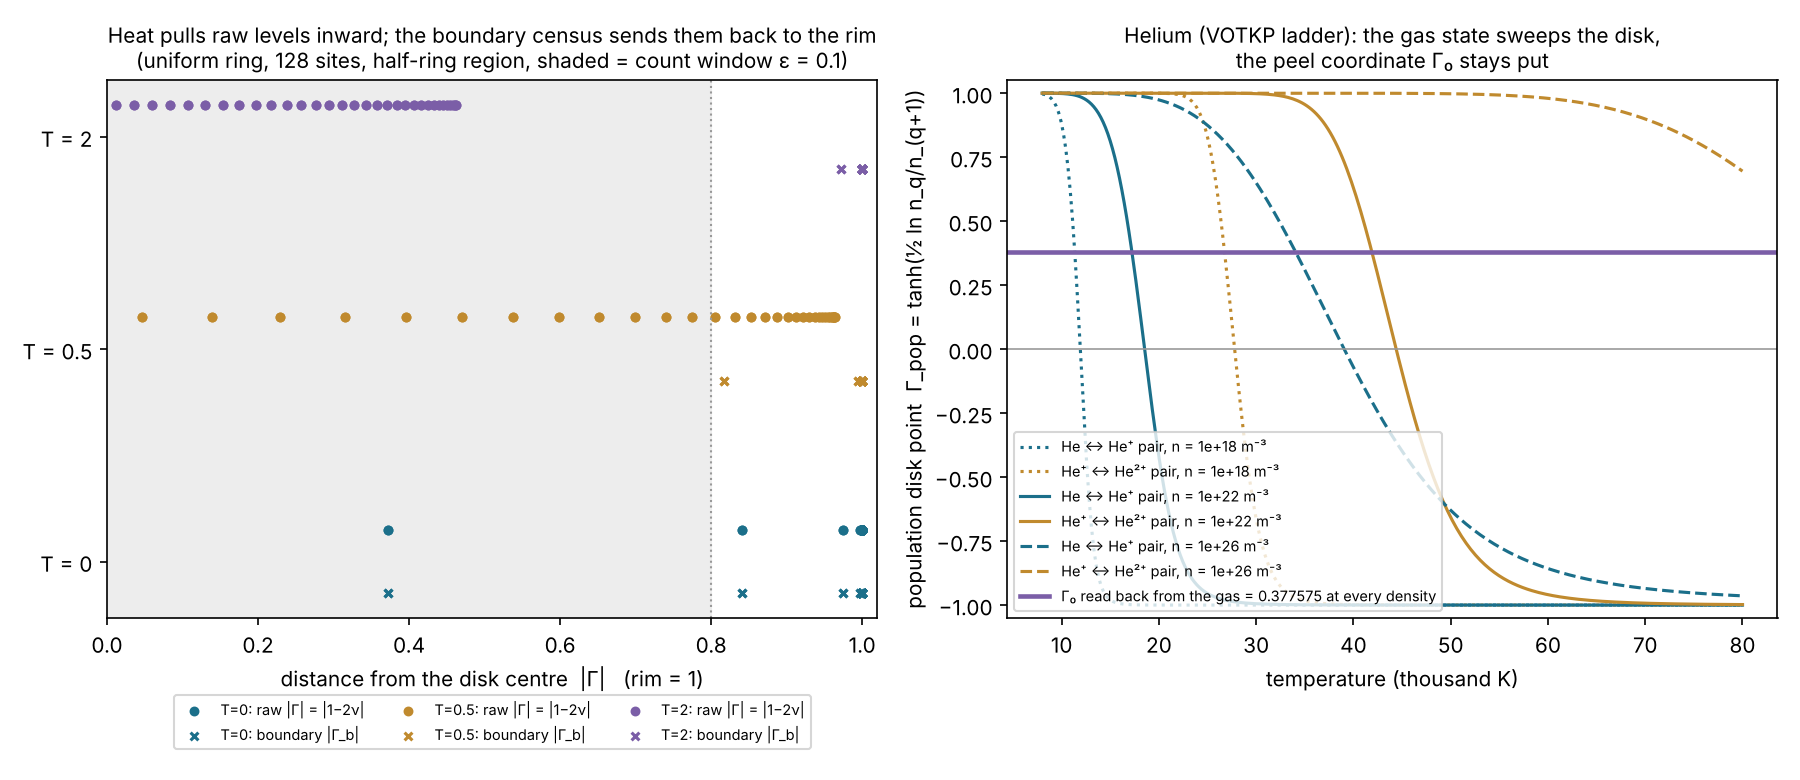
\includegraphics[width=\textwidth]{fig02_boundary_and_gas.png}
\caption{Left: heat pulls raw census levels toward the centre of the disk; the boundary coordinate $|\Gamma_b|$ keeps only what crosses the cut. Right: helium's charge-state pairs sweep the disk as the gas changes, while $\Gamma_0$ read back from the gas stays at $0.377575$.}
\label{fig:boundary}
\end{figure}

\section{One chart for all of it}
\begin{theorem}[peel steps add like velocities; VOTKP Theorem 15.1]\label{thm:add}
For a positive ladder $I_0,\dots,I_n$ with steps $\Gamma_k=\tanh(\tfrac12\ln(I_{k+1}/I_k))$, the composite of a block of steps is $\Gamma_{j\to l}=\Gamma_j\oplus\Gamma_{j+1}\oplus\dots\oplus\Gamma_{l-1}$, with $u\oplus v=(u+v)/(1+uv)$. \grade{T}
\end{theorem}
\begin{proof}
$\ln(I_l/I_j)=\sum_k\ln(I_{k+1}/I_k)$, and $\tanh(a+b)=\tanh a\oplus\tanh b$.
\end{proof}
This is Einstein's addition of collinear velocities; the half-rapidities add. On the Smith disk read as the Poincaré disk the peel is a walk along a geodesic diameter whose hyperbolic lengths add (VOTKP Corollary 15.2) \grade{T}. The composite forgets the order of its steps; the resolved ladder keeps it.

\paragraph{Matter's census ladder is a peel ladder.} On the transverse-field Ising chain ($c=\tfrac12$) the single-particle entanglement energies are odd multiples $\varepsilon_0,3\varepsilon_0,5\varepsilon_0,\dots$ of one spacing (\emph{Matter at a Scale}, LADDER-C12-01). By Theorem~\ref{thm:add} the levels then satisfy $\Gamma_{j+1}=\Gamma_j\oplus\tanh\varepsilon_0$: one constant peel step. Measured residuals are $8.0\times10^{-6}$, $5.5\times10^{-6}$, $3.2\times10^{-6}$ at $\xi=20.5$, $50.5$, $125.5$, and the ladder's own uniformity error falls $0.022$, $0.011$, $0.0062$ \grade{V} (script \texttt{s02}). Near the rim the disk compresses differences, so the informative number is the uniformity error in rapidity.

\begin{figure}[t]\centering
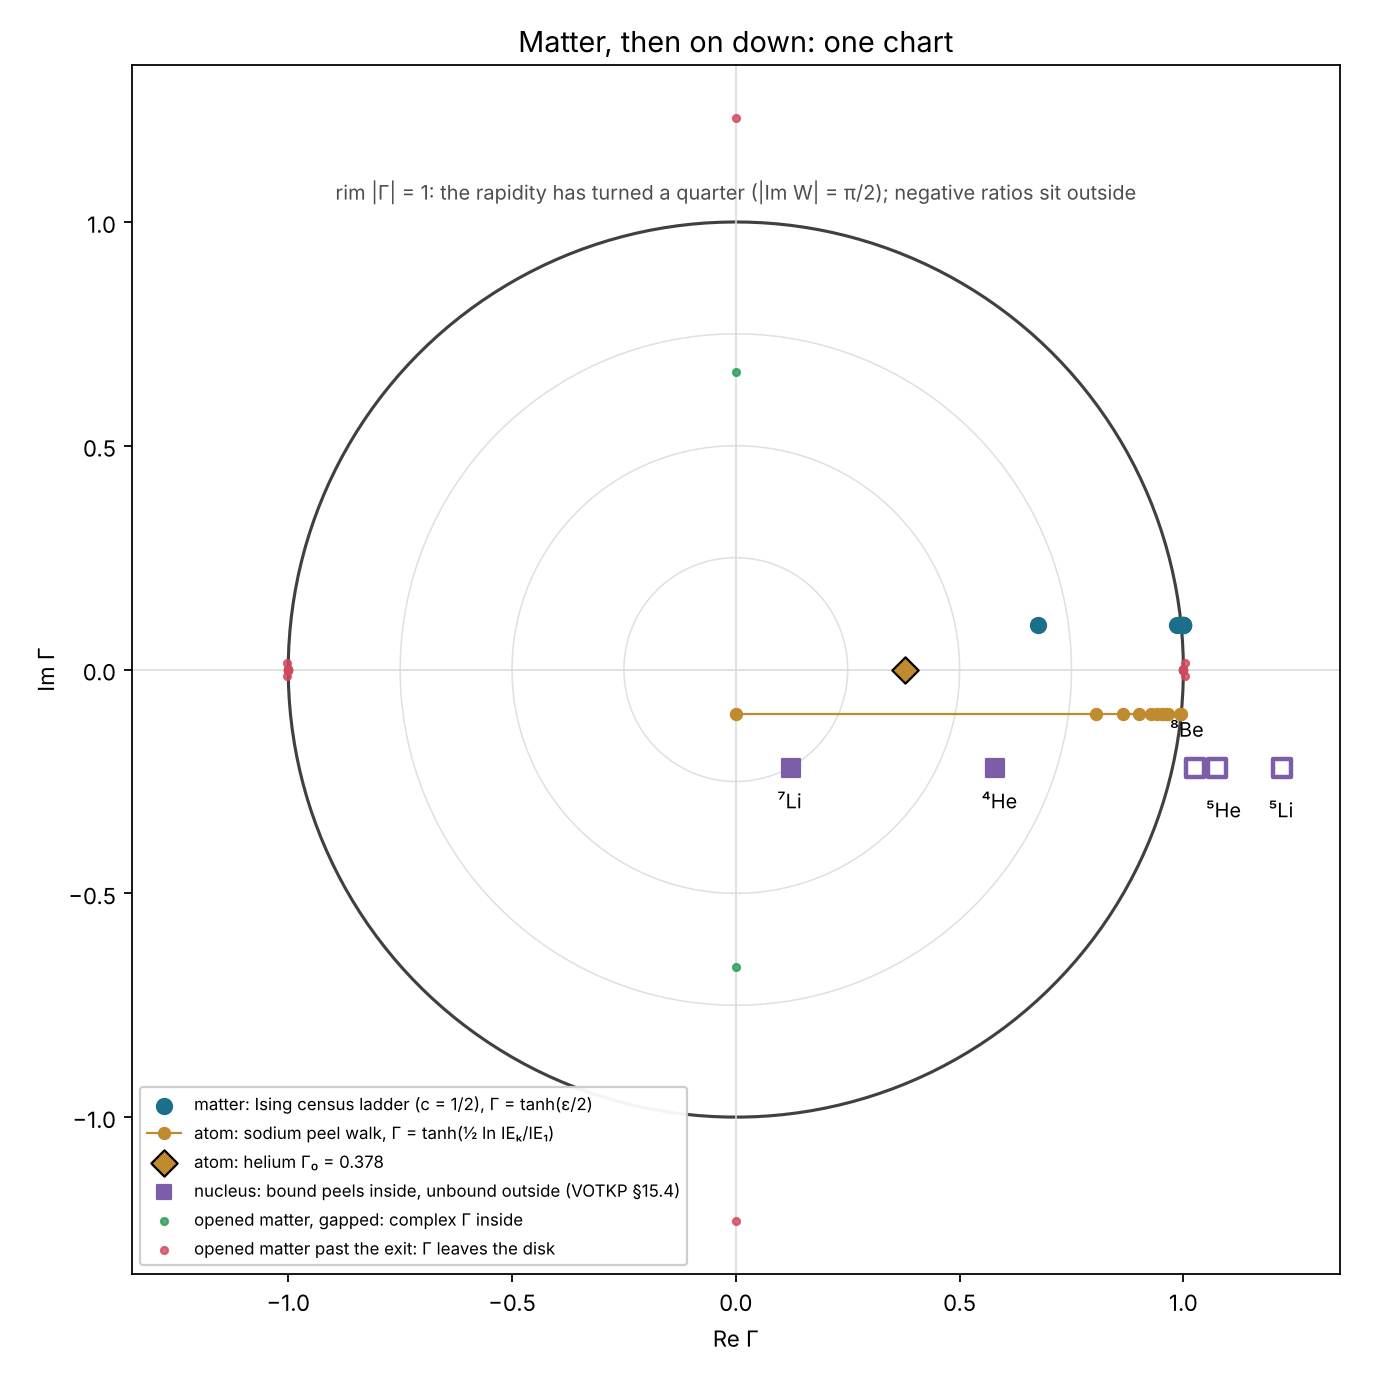
\includegraphics[width=0.82\textwidth]{fig03_matter_then_down.png}
\caption{One chart, every scale. Blue: the Ising census ladder, $\Gamma=\tanh(\varepsilon/2)$. Gold: sodium's peel walk $\tanh(\frac12\ln I_k/I_1)$ from NIST thresholds, and helium's $\Gamma_0$. Purple: nuclear separation-energy peels; bound nuclei inside, the unbound mass-5 and mass-8 gaps outside (VOTKP §15.4, recomputed from NUBASE2020). Green and red: census levels of the opened non-Hermitian SSH chain ($u=0.5$) before ($v=0.30$) and past ($v=0.49$) its exit.}
\label{fig:hero}
\end{figure}

\section{The atom}
For an atom the ratio is between successive relaxed removal thresholds, $z_q=I_{q+1}/I_q$, and every step lies on the positive real radius (VOTKP §8, Theorem 8.1 chart). Helium's two thresholds, $24.587389011$ and $54.4177655282$\,eV, give $\Gamma_0=0.377575066984$ and a binding sum of $79.0051545392$\,eV \grade{T}. An anchor and the full coordinate vector reconstruct the ladder exactly, $I_q=I_0\prod_{j<q}(1+\Gamma_j)/(1-\Gamma_j)$, and a common scale leaves every $\Gamma$ unchanged \grade{T}. VOTKP Theorem 15.4 (scale blindness) is the atomic form of §1: multiplying every mass by $\lambda$ scales every energy by $\lambda$ and leaves every ratio fixed, so the peel coordinate is blind to which particle carries the charge except through charges, mass ratios and statistics \grade{T}. The coordinate needs a physical zero: removal energies are measured from the continuum, which is why the ratio means something, and why quantum-dot addition spectra, which can be moved up or down, have no peel (VOTKP §15.3).

Sodium's eleven thresholds walk from the centre to $\Gamma=0.9938$ along one diameter (Figure~\ref{fig:hero}); shell jumps are the long strides. The last peel step is derived in closed form (VOTKP §15.10), and the middle of the peel follows the Thomas–Fermi law with $\Gamma_k\to\tanh(\tfrac23\ln\tfrac{k+1}{k})\approx2/(3k)$ (§15.11, cited there) \grade{T}/\grade{lit}.

\section{The nucleus}
A nucleus peels by separation energies. VOTKP §15.4 uses $z=S_{\mathrm{next}}/S_{\mathrm{first}}$ and the same $\Gamma$, ``the form that extends to $z<0$''. A bound peel has $z>0$ and sits inside the disk. A negative separation energy gives $z<0$ and $|\Gamma|>1$; $z=-1$ is a Cayley pole, and the real logarithmic rapidity is not extended across it. Recomputed here from NUBASE2020 with the author's own script:

\begin{center}
\begin{tabular}{lrrrl}\toprule
case & $S_{\mathrm{first}}$ (keV) & $S_{\mathrm{next}}$ (keV) & $|\Gamma|$ & half-life\\\midrule
${}^5$He: $n$, then $n$ from ${}^4$He & $-734.8$ & $20577.6$ & $1.074$ & 602 ys\\
${}^5$Li: $p$, then $p$ from ${}^4$He & $-1966.1$ & $19813.9$ & $1.220$ & 370 ys\\
${}^8$Be: $\alpha$ ($^{12}$C ladder) & $-91.8$ & $7366.6$ & $1.025$ & 81.9 as\\
${}^7$Li (bound) & $7251.1$ & $5664.4$ & $0.123$ & stable\\
${}^4$He (bound) & $20577.6$ & $5493.5$ & $0.579$ & stable\\\bottomrule
\end{tabular}
\end{center}
\noindent These agree with VOTKP §15.4 to every printed digit \grade{V}\grade{lit}.

\paragraph{How far outside, exactly.} VOTKP §15.4 notes that the distance outside the rim is close to twice the decay energy over the neighbouring step. It is exact in this form. Write $S_{\mathrm{first}}=-s<0$ and $a=S_{\mathrm{next}}/s>1$, so $z=-a$ and
\[
|\Gamma|=\frac{a+1}{a-1},\qquad |\Gamma|-1=\frac{2}{a-1}=\frac{2s}{S_{\mathrm{next}}-s},
\]
which is $2s/S_{\mathrm{next}}$ when $s\ll S_{\mathrm{next}}$ \grade{T}. On the three gap nuclei the identity holds exactly ($0.074062$, $0.220318$, $0.025238$), against the small-$s$ values $0.071417$, $0.198457$, $0.024923$ (script \texttt{s12}). The Cayley pole $z=-1$ is $S_{\mathrm{first}}+S_{\mathrm{next}}=0$. The placement says no more than the sign of a separation energy, and the author's own caution stands: a resonance's leak through its barrier ``is not a literal atomic or nuclear Smith reflection derived from the threshold coordinate''.

\paragraph{The half-turn.} Write $\Gamma=\tanh(W/2)$ with $W=\operatorname{Log}z$ (principal branch). For $z\neq-1$, $|z+1|^2-|z-1|^2=4\operatorname{Re}z$, so $|\Gamma|<1\iff\operatorname{Re}z>0\iff|\operatorname{Im}W|<\pi/2$ \grade{T}. A negative ratio has $\operatorname{Im}W=\pi$ exactly: the three unbound nuclei are peels whose rapidity has turned half a revolution, and the rim of the disk is the quarter-turn. Random complex $z$ ($4000$ draws) give zero mismatches, and $z=-28$ gives $\Gamma=1.0741$, the ${}^5$He value \grade{V} (script \texttt{s04a}). A complex ratio by itself does not leave the disk: $z=1-i\gamma$ stays inside for every $\gamma$, since $\operatorname{Re}z>0$. Leaving needs a ratio whose real part changes sign.

\section{Opened matter}
\subsection{The opened chain}
Opening matter means a non-Hermitian generator. The cone paper (v8) proves that at a Hermitian point the round-trip form $Q(\theta)=M_{+-}M_{-+}/(E_+-E_-)^2$ has $\operatorname{Re}Q\ge0$, so no cone exists there, and measures a Lorentzian cone when the system is opened \grade{T}/\grade{V}. Take the PT-symmetric SSH chain
\[
h(k)=\begin{pmatrix} iu & v+we^{-ik}\\ v+we^{ik} & -iu\end{pmatrix},\qquad E(k)^2=|v+we^{ik}|^2-u^2,
\]
fill the lower band with the biorthogonal projector, and restrict to a block. The occupations are complex, and so is $\Gamma=1-2\nu$; the biorthogonal $C$ is still idempotent ($\|C^2-C\|\le3\times10^{-14}$), so $Y_A=C_{AB}C_{BA}=C_A-C_A^2$ and the radial census $\sqrt{|1-4\lambda|}=|1-2\nu|$ survive opening \grade{T}\grade{V}. On the opened plane at $u=0.5$ the band metric is Lorentzian over $93\%$ of the cells, its determinant changes sign exactly at the critical points $|v-w|=u$, and the closed plane is degenerate \grade{V}. At the critical point the Rényi-2 central charge reads $-1.79\to-1.96$ on the $v<w$ side \grade{V}; the $v>w$ side has not converged. A negative fitted coefficient is a property of the biorthogonal entropy convention, not a negative number of channels.

\subsection{Where opened matter leaves the disk}
Approaching the critical point at fixed $u$, the census levels leave the disk \emph{before} it, inside the gapped phase, and the exit does not move under a fourfold larger block or a doubled ring ($v_{\mathrm{exit}}=0.468$ at $u=0.5$) \grade{V}. At every critical point tested ($u=0.2,\dots,0.7$) a level sits at $\operatorname{Im}W=\pi$ exactly: the half-turn of the unbound nuclei.

\begin{proposition}[the exit line of the PT-symmetric chain]
The Petermann factor of the lower band is $K(k)=1+u^2/E(k)^2$, and for $A=v^2+w^2-u^2>|2vw|$ its band average is
\[
\langle K\rangle=1+\frac{u^2}{\sqrt{A^2-B^2}}=1+\frac{u^2}{E(0)E(\pi)},\qquad B=2vw.
\]
Hence $\langle K\rangle=2\iff E(0)E(\pi)=u^2$. \grade{T}
\end{proposition}
\begin{proof}
For $h=d\cdot\sigma$ with $E^2=d\cdot d$ the band projector is $P=\tfrac12(I-h/E)$ and $K=\Tr P^\dagger P=\tfrac12(1+\sum|d_j|^2/|E|^2)$. Here $d=(\operatorname{Re}q,\operatorname{Im}q,iu)$, so $\sum|d_j|^2=|q|^2+u^2$ and $|E|^2=|q|^2-u^2$, giving $K=1+u^2/E^2$. With $E^2=A+B\cos k$ and $\frac1{2\pi}\int_0^{2\pi}\frac{dk}{A+B\cos k}=\frac1{\sqrt{A^2-B^2}}$, and $\sqrt{A^2-B^2}=\sqrt{A+B}\sqrt{A-B}=E(0)E(\pi)$.
\end{proof}
Checked to $3.6\times10^{-14}$. Predicted from $\langle K\rangle=2$ at three values of $u$ not used before, the exits are $0.7474014$, $0.5291503$, $0.2357262$; measured, $0.7474015$, $0.5291503$, $0.2357262$ (differences $4\times10^{-8}$ and below) \grade{V}.

\paragraph{The limits of the exit law.} Three findings scope it, and they belong in the statement.
\begin{enumerate}
\item On the cone paper's band made one-dimensional, $d=(t_1+\cos k,\sin k,m+i\gamma)$, a mass term moves the exit far earlier ($\langle K\rangle\approx1.015$–$1.022$); the law holds only at $m=0$, which is the SSH class \grade{V}.
\item The massive exit depends on the endpoint filter that discards levels with $\nu$ at $0$ or $1$: $\gamma_{\mathrm{exit}}=0.27164$ at filters $10^{-6}$ and $10^{-8}$, $0.16917$ at $10^{-9}$ and $10^{-10}$, $0.12272$ at $10^{-12}$, while the massless exit stays at $0.47434$ through $10^{-8}$ \grade{V}. This was found in an independent formal review (3 November 2026) and reproduced here (script \texttt{s09}).
\item With $w=0$ and $v^2=2u^2$ the band average is exactly 2, yet no block level ever leaves $\{0,1\}$ \grade{T}. So the average alone does not force an exit; the coupling and the partition are part of the law.
\end{enumerate}
What survives: on the coupled PT-symmetric chain with whole-cell blocks and the stated filter, the census leaves the disk where $E(0)E(\pi)=u^2$, to $4\times10^{-8}$ \grade{V}; why it does is open \grade{C}.

\subsection{The offset as the exit's clock}
For opened matter each level's offset $\tau_\nu=\operatorname{Log}((1-\nu)/\nu)$ is complex, and the rotation used above is $|\operatorname{Im}\tau_\nu|/\pi$. The disk exit is the place where some level's signed offset has turned a quarter, and the critical point the place where one has turned a half.

The author's closed form for the endpoint offset of a gapped chain, $2\operatorname{artanh}(v/\sqrt{E_{\min}E_{\max}})$ (\emph{The Offset Belongs to the Boundary}), continued to the opened chain, has imaginary part $\operatorname{Im}\tau=2\arctan\big(u/\sqrt{E(0)E(\pi)}\big)$. Then exactly
\[
\langle K\rangle=1+\frac{u^2}{E(0)E(\pi)}=\sec^2\!\Big(\tfrac12\operatorname{Im}\tau\Big),
\]
so $\langle K\rangle=2$ is the same statement as $\operatorname{Im}\tau=\pi/2$: the exit law of §6.2 is a quarter-turn of this offset \grade{T}. It is not, however, a description of the census rotation away from the exit. Tested before the run with a kill condition, at $u=0.3,0.5,0.7$ and three points on the approach, the measured rotation sits $4\times10^{-6}$ to $3.4\times10^{-2}$ above the formula, independent of block size; the two meet only at the quarter-turn. The level that carries the largest rotation is often one with $\nu$ within $10^{-7}$ of an endpoint, the same ill-conditioned levels as the filter result above \grade{V}. Whether a biorthogonal form of the speed limit $\dot\tau^2\le4gS$ governs the rotation is open \grade{C}.

\section{What is proved, what is measured, what is open}
\begin{center}\small
\begin{tabular}{p{0.62\textwidth}l}\toprule
Statement & grade\\\midrule
Zero and span free; census logarithm with $A=2c/\pi^2$ & \grade{T}, \grade{V} at $c=1,\tfrac12$\\
$\Gamma=\tanh(\varepsilon/2)=1-2\nu$; $\int H\,d\varepsilon=\pi^2/3$ & \grade{T}\\
Offset = summed level rapidity = log-odds empty/full & \grade{T}\\
$\Gamma_b=|1-2\nu|$; $\Tr X_A=$ the weight between & \grade{T}\\
Offset speed limit $\dot\tau^2\le4gS$ & \grade{T}\\
Warm census: heat moves raw levels, not boundary levels (ring, 128 sites) & \grade{V}\\
Ising census ladder = constant peel step & \grade{V}\\
Peel steps add like velocities & \grade{T}\\
Ideal helium gas returns $\Gamma_0$ at every density & \grade{R}\\
Unbound nuclei outside the disk; half-turn of the rapidity & \grade{T}, \grade{V}\grade{lit}\\
Rim distance $|\Gamma|-1=2s/(S_{\mathrm{next}}-s)$ & \grade{T}\\
$\langle K\rangle=\sec^2(\tfrac12\operatorname{Im}\tau)$: exit = quarter-turn of the offset & \grade{T}\\
Biorthogonal idempotence; radial census survives opening & \grade{T}, \grade{V}\\
Opened matter exits before critical; exit line $E(0)E(\pi)=u^2$ (PT class, stated filter and partition) & \grade{V}\\
$\langle K\rangle=1+u^2/(E(0)E(\pi))$ & \grade{T}\\\bottomrule
\end{tabular}
\end{center}
\noindent Open: why the census rotation meets the offset quarter-turn only at the exit, which needs conditioned eigenvalues for the near-endpoint levels; a proof that the exit happens exactly at $\langle K\rangle=2$ on the coupled chain; a filter-independent definition of the massive exit (filter, ring and block sizes, order of limits); a biorthogonal speed limit for the complex offset; convergence on the $v>w$ side; placing nuclear resonances with their widths on the chart; a second non-unitary model of a different kind.

\section*{Sources}
\small
J.~Beasley, \emph{Matter at a Scale: Zero, Span, and the Logarithm Between Them}, v5 (2026), doi:10.5281/zenodo.22019893.
J.~Beasley, \emph{VOTKP: The Vector of Traits Kept under Peeling}, v2.9 (2026), doi:10.5281/zenodo.23340757.
J.~Beasley, \emph{The Offset Belongs to the Boundary}, v31 (2026), doi:10.5281/zenodo.22555919.
J.~Beasley, \emph{The Offset Speed Limit}, v1.1 (2026).
J.~Beasley, \emph{The Weight Between}, v2.3 (2026).
J.~Beasley, \emph{The Angle Between the Rails} (2026).
J.~Beasley, \emph{A Measured Lorentzian Cone in Non-Hermitian Quantum Geometry}, v8 (2026).
J.~Beasley, \emph{Beyond the Event Horizon}, edition 10 (2026).
F.~G.~Kondev et al., The NUBASE2020 evaluation of nuclear physics properties, Chin.\ Phys.\ C 45 (2021) 030001.
A.~Kramida et al., NIST Atomic Spectra Database (ionization energies), accessed through the VOTKP v2.9 package.
P.-Y.~Chang, J.-S.~You, X.~Wen, S.~Ryu, Phys.\ Rev.\ Research 2 (2020) 033069.
Independent formal review, \emph{Matter, Gases and VOTKP}, 3 November 2026 (prepared with OpenAI tools), kept in the repository.
\normalsize

\appendix
\section{Proofs of every result used}
This appendix makes the paper standalone. Each result used in the text is restated and proved here, including those taken from the author's earlier papers. Where a proof rests on an outside input, the input is named and is the only thing assumed. Items marked \textsf{[Lean]} are also checked by machine (Appendix B).

\paragraph{A.1 Zero and span are free (§1).}
\emph{Statement.} For a Hermitian generator $K$, a shift $K\mapsto K+cI$ leaves every eigenvector and every eigenvalue difference unchanged, and a positive rescaling $K\mapsto cK$, $c>0$, leaves every eigenvector, the order of the eigenvalues, every spectral projector $\mathbf 1[K<0]$, and so the ground-state correlation matrix and its census, unchanged.
\emph{Proof.} $K+cI$ commutes with $K$ and has eigenvalues $\lambda_i+c$, so $\lambda_i-\lambda_j$ is unchanged. $cK$ has the same eigenvectors with eigenvalues $c\lambda_i$; since $c>0$, $c\lambda_i<0\iff\lambda_i<0$, so the filled projector $P=\mathbf 1[K<0]$ is the same operator. The regional correlation matrix $C_A=E^\dagger PE$ and every function of its spectrum, including the census, are therefore unchanged; so are principal angles between spectral subspaces, which depend only on the subspaces. \qed

\paragraph{A.2 The census coefficient $A=2c/\pi^2$ (§1, eq.~\ref{eq:census}).}
\emph{Inputs.} (i) The single-particle entanglement spectrum at one cut is equally spaced, $\varepsilon_j=(j+\tfrac12)\Delta$ on both signs, as measured on the Ising chain (§3, script \texttt{s02}) and derived in \emph{The Angle Between the Rails}. (ii) The entanglement entropy of one cut in a gapped chain near criticality is $S_{\mathrm{cut}}=\tfrac c6\ln(\xi/a)+O(1)$ (Calabrese–Cardy).
\emph{Derivation.} A level is in the window $\nu\in[\epsilon,1-\epsilon]$ iff $|\varepsilon|\le\Lambda=\ln((1-\epsilon)/\epsilon)=\ln(1/\epsilon)+O(\epsilon)$ (Proposition~\ref{prop:bridge}). With spacing $\Delta$ on both signs, one cut has $N_{\mathrm{cut}}=2\Lambda/\Delta+O(1)$ levels in the window. Its entropy is $S_{\mathrm{cut}}=\sum_jH(\nu(\varepsilon_j))=\Delta^{-1}\int H\,d\varepsilon+O(\Delta)=\pi^2/(3\Delta)+O(\Delta)$ by Proposition~\ref{prop:bridge} (midpoint rule). Equating with (ii), $1/\Delta=(c/2\pi^2)\ln(\xi/a)$, so $N_{\mathrm{cut}}=(c/\pi^2)\ln(\xi/a)\ln(1/\epsilon)$, and an interval with two cuts has $A=2c/\pi^2$. \qed\ The derivation is exact given (i) and (ii); its corrections are those of the two inputs.

\paragraph{A.3 The bridge, and $\int H\,d\varepsilon=\pi^2/3$ (Proposition~\ref{prop:bridge}).}
Proved in the text. The last step uses $\int_0^1(-\ln\nu)/(1-\nu)\,d\nu=\sum_{n\ge0}\int_0^1\nu^n(-\ln\nu)\,d\nu=\sum_{n\ge1}n^{-2}=\pi^2/6$, and $\int_0^1H/(\nu(1-\nu))\,d\nu=2\int_0^1(-\ln\nu)/(1-\nu)\,d\nu$ by the symmetry $\nu\leftrightarrow1-\nu$ and $H/(\nu(1-\nu))=-\ln\nu/(1-\nu)-\ln(1-\nu)/\nu$. The identities $\Gamma=1-2\nu$ and $\nu(1-\nu)=(1-\Gamma^2)/4$ \textsf{[Lean: \texttt{bridge}, \texttt{census\_square}]}.

\paragraph{A.4 The offset is the log-odds of empty against full (§2.1; \emph{The Offset Belongs to the Boundary}, Thm 2).}
\emph{Statement.} For a number-conserving Gaussian fermion state with $0<C_A<I$, $\tau=\Tr[\log(I-C_A)-\log C_A]=\log\det(I-C_A)-\log\det C_A=\log P(N_A=0)/P(N_A=|A|)$.
\emph{Proof.} The reduced state of a Gaussian state is Gaussian, $\rho_A\propto\exp(-\sum_k\varepsilon_kb_k^\dagger b_k)$ in the eigenmodes $b_k$ of $C_A$, so it is a product over modes with occupation $\nu_k=1/(1+e^{\varepsilon_k})$. The region is empty iff every mode is empty and full iff every mode is filled, so $P(0)=\prod_k(1-\nu_k)=\det(I-C_A)$ and $P(|A|)=\prod_k\nu_k=\det C_A$. Taking logs, $\tau=\sum_k\ln((1-\nu_k)/\nu_k)=\sum_k\varepsilon_k$. The example in the text: $\mathrm{diag}(0.2,0.8)$ gives $\ln4+\ln\tfrac14=0$, $\mathrm{diag}(0.2,0.2)$ gives $2\ln4=\ln16$, while both have $C-C^2=0.16I$. \qed

\paragraph{A.5 Defect split and the weight between (§2.2).}
\emph{Statement.} Write $C=\begin{pmatrix}C_A&C_{AB}\\C_{BA}&C_B\end{pmatrix}$. Then $(C^2)_{AA}=C_A^2+C_{AB}C_{BA}$, so $C_A-C_A^2=(C-C^2)_{AA}+X_A$ with $X_A=C_{AB}C_{BA}$. If $C^2=C$ then $X_A=C_A-C_A^2$, with no Hermiticity used. If $C$ is Hermitian, $\Tr X_A=\|C_{AB}\|_F^2=\|P_AC(1-P_A)\|_F^2$.
\emph{Proof.} Block multiplication gives the first identity \textsf{[Lean: \texttt{topleft\_sq}]}; subtracting it from $C_A$ gives the split. If $C^2=C$ the first term vanishes \textsf{[Lean: \texttt{idempotent\_cross}]}. For Hermitian $C$, $C_{BA}=C_{AB}^\dagger$, so $\Tr C_{AB}C_{AB}^\dagger=\|C_{AB}\|_F^2$, and $P_AC(1-P_A)$ is $C_{AB}$ padded with zeros. With $H$ in place of $C$ this is the coupling energy $E_B=\|PH(1-P)\|_F^2$ of \emph{The Weight Between}. \qed

\paragraph{A.6 The boundary coordinate is the modulus (§2.2), and it survives opening (§6.1).}
\emph{Statement.} If $C^2=C$, each eigenvalue $\lambda$ of $X_A$ is $\nu(1-\nu)$ for an eigenvalue $\nu$ of $C_A$, and $\sqrt{|1-4\lambda|}=|1-2\nu|$. This holds for the biorthogonal projector $C=\sum_{k\,\mathrm{filled}}|R_k\rangle\langle L_k|$ with $\langle L_j|R_k\rangle=\delta_{jk}$.
\emph{Proof.} By A.5, $X_A=C_A-C_A^2=f(C_A)$ with $f(x)=x-x^2$, so by the spectral mapping theorem (valid for any square matrix, via the Jordan form) its eigenvalues are $f(\nu)$. Then $1-4f(\nu)=(1-2\nu)^2$ \textsf{[Lean: \texttt{census\_square}]}, whose modulus has square root $|1-2\nu|$ for complex $\nu$ too. For the biorthogonal projector, $C^2=\sum_{j,k}|R_j\rangle\langle L_j|R_k\rangle\langle L_k|=C$. \qed

\paragraph{A.7 The Offset Speed Limit (§2.2; \emph{The Offset Speed Limit}, Thm 1 and Cor.~3).}
\emph{Statement.} Let $P(t)$ be a smooth family of orthogonal projectors on $\mathbb C^n$, $E$ an $n\times m$ isometry onto the region, $C=E^\dagger PE$ with $0<C<I$, $\tau=\Tr[\log(I-C)-\log C]$, $g=\tfrac12\|\dot P\|_F^2$ and $S=\Tr[(C(I-C))^{-1}]$. Then $\dot\tau^2\le4gS$, with equality iff $\dot P$ is a real multiple of $T=[P,[P,F]]$, $F=EWE^\dagger$, $W=-(C(I-C))^{-1}$. If $\dot P=-i[H,P]$ then $g=E_B$ and $|\dot\tau|\le2\sqrt{E_BS}$.
\emph{Proof.} \emph{Step 1 (trace derivative).} $\frac{d}{dt}\Tr\log(I-C)=-\Tr[(I-C)^{-1}\dot C]$ and $\frac d{dt}\Tr\log C=\Tr[C^{-1}\dot C]$; since $(I-C)^{-1}+C^{-1}=(C(I-C))^{-1}$, $\dot\tau=\Tr[W\dot C]$. \emph{Step 2 (lift).} $\dot C=E^\dagger\dot PE$, so $\dot\tau=\Tr[EWE^\dagger\dot P]=\Tr[F\dot P]$, with $F$ Hermitian. \emph{Step 3 (only the off-diagonal part counts).} Differentiating $P^2=P$ gives $\dot PP+P\dot P=\dot P$, hence $P\dot PP=0$ and $(1-P)\dot P(1-P)=0$: $\dot P$ is block off-diagonal. So $\Tr[F\dot P]=\Tr[F_{\mathrm{off}}\dot P]$ with $F_{\mathrm{off}}=PF(1-P)+(1-P)FP$, and expanding, $[P,[P,F]]=PF+FP-2PFP=F_{\mathrm{off}}=T$. \emph{Step 4 (Cauchy–Schwarz).} In the Hilbert–Schmidt inner product, $\dot\tau^2=\langle T,\dot P\rangle^2\le\|T\|_F^2\|\dot P\|_F^2=2g\|T\|_F^2$, with equality iff $\dot P=\lambda T$, $\lambda\in\mathbb R$. \emph{Step 5 ($\|T\|_F^2=2S$).} $\|T\|_F^2=2\Tr[PF(1-P)FP]=2\Tr[W\,E^\dagger(1-P)E\,W\,E^\dagger PE]=2\Tr[W(I-C)WC]=2\Tr[W^2C(I-C)]=2S$, because $W$, $C$ and $I-C$ commute. Hence $\dot\tau^2\le4gS$. For the corollary, $[H,P]=(1-P)HP-PH(1-P)$, whose two blocks are adjoint up to sign, so $\|\dot P\|_F^2=2\|PH(1-P)\|_F^2$ and $g=E_B$. \qed

\paragraph{A.8 Peel steps add like velocities (Theorem~\ref{thm:add}; VOTKP Thm 15.1).}
Proved in the text. In the division-free form used by the Lean file, $g(z_1)+g(z_2)=g(z_1z_2)\,(1+g(z_1)g(z_2))$ for $z_1,z_2>0$, with $g(z)=(z-1)/(z+1)$ \textsf{[Lean: \texttt{rapidities\_add}]}. Since $1+g_1g_2>0$ for $|g_i|<1$, this is $g(z_1z_2)=g_1\oplus g_2$. The ladder reconstruction $I_q=I_0\prod_{j<q}(1+\Gamma_j)/(1-\Gamma_j)$ is the inverse $z=(1+\Gamma)/(1-\Gamma)$ applied step by step.

\paragraph{A.9 Scale blindness (§4; VOTKP Thm 15.4).}
\emph{Statement.} For a nonrelativistic Coulomb system $H_\lambda=\sum_i p_i^2/(2\lambda m_i)+\sum_{i<j}q_iq_j/|r_i-r_j|$, multiplying every mass by $\lambda>0$ multiplies every energy by $\lambda$, so every ratio of removal energies, and every $\Gamma$, is unchanged.
\emph{Proof.} Let $U$ be the unitary dilation $(U\psi)(r)=\lambda^{3N/2}\psi(\lambda r)$. Then $U^\dagger r_iU=r_i/\lambda$ and $U^\dagger p_iU=\lambda p_i$, so $U^\dagger H_\lambda U=\sum_i\lambda^2p_i^2/(2\lambda m_i)+\lambda\sum_{i<j}q_iq_j/|r_i-r_j|=\lambda H_1$. Unitarily equivalent operators have the same spectrum, so $\mathrm{spec}\,H_\lambda=\lambda\,\mathrm{spec}\,H_1$, and so do the thresholds of every ion, which are bottoms of spectra of subsystems. Ratios cancel $\lambda$. \qed\ Mass \emph{ratios} still enter, which is why the ${}^1$H/${}^2$H isotope shift is visible (VOTKP §15.3).

\paragraph{A.10 The last peel step at first order (§4; VOTKP §15.10).}
\emph{Statement.} To first order in the electron repulsion, a helium-like ion of charge $Z$ has removal threshold $I_{\mathrm{He}}=Z^2/2-5Z/8$ Hartree, the hydrogen-like ion $I_{\mathrm H}=Z^2/2$, and the last step has $\Gamma=5/(8Z-5)\to5/(8Z)$.
\emph{Proof.} The hydrogen-like ground energy is $-Z^2/2$. Two non-interacting $1s$ electrons have $-Z^2$. The first-order repulsion is $J=\iint\rho(r_1)\rho(r_2)/|r_1-r_2|$ with $\rho=(Z^3/\pi)e^{-2Zr}$. By Gauss's law the potential of $\rho$ is $\phi(r)=1/r-(Z+1/r)e^{-2Zr}$, so
\[
J=4Z^3\!\int_0^\infty\! r^2e^{-2Zr}\phi(r)\,dr=4Z^3\Big[\tfrac1{4Z^2}-\tfrac{2Z}{(4Z)^3}-\tfrac1{(4Z)^2}\Big]=4Z^3\cdot\tfrac{10}{64Z^2}=\tfrac58Z
\]
(Unsöld 1927). So $E_{\mathrm{He}}=-Z^2+5Z/8$ and $I_{\mathrm{He}}=-Z^2/2-E_{\mathrm{He}}=Z^2/2-5Z/8$. With $z=I_{\mathrm H}/I_{\mathrm{He}}$, $\Gamma=(I_{\mathrm H}-I_{\mathrm{He}})/(I_{\mathrm H}+I_{\mathrm{He}})=(5Z/8)/(Z^2-5Z/8)=5/(8Z-5)$ \textsf{[Lean: \texttt{last\_step}]}. \qed\ The higher terms of the $1/Z$ series (Hylleraas; Scherr–Knight) are cited inputs in VOTKP and are not used here. The Thomas–Fermi middle of the peel (§15.11) is cited there as an external result and is not proved in this paper.

\paragraph{A.11 Ideal Saha gas: the electron density cancels (§2.4).}
\emph{Input.} The ideal Saha equation $n_{i+1}n_e/n_i=(2g_{i+1}/g_i)\lambda_e^{-3}e^{-\beta I_i}$ with constant statistical weights.
\emph{Statement.} $n_0n_2/n_1^2=(g_0g_2/g_1^2)\,e^{-\beta(I_1-I_0)}$ and $n_0/(n_2n_e^2\lambda_e^6)=(g_0/4g_2)\,e^{\beta(I_0+I_1)}$, independent of density; their $\beta$-slopes return $I_1-I_0$ and $I_0+I_1$, hence $\Gamma_0=(I_1-I_0)/(I_1+I_0)$.
\emph{Proof.} Divide the $i=1$ equation by the $i=0$ one: $n_e$ and $\lambda_e$ cancel \textsf{[Lean: \texttt{saha\_ratio}, the cancellation step]}. Multiply the two equations for the second form. The ratio of the two slopes gives $\Gamma_0$. \qed\ With temperature-dependent partition functions the slopes acquire $d\ln g/d\beta$ terms, which is the bias stated in §2.4.

\paragraph{A.12 Outside the rim, exactly, and the Cayley pole (§5).}
For $S>s>0$ and $z=S/(-s)$: $\Gamma=(S+s)/(S-s)$ and $\Gamma-1=2s/(S-s)$; $S_2/S_1=-1\iff S_1+S_2=0$ \textsf{[Lean: \texttt{outside\_rim}, \texttt{rim\_distance}, \texttt{cayley\_pole}]}. The half-turn statement $|\Gamma|<1\iff\operatorname{Re}z>0$ is proved in the text from $|z+1|^2-|z-1|^2=4\operatorname{Re}z$; and $\operatorname{Re}z>0\iff|\operatorname{Im}\operatorname{Log}z|<\pi/2$ because $\operatorname{Re}z=|z|\cos(\operatorname{Im}\operatorname{Log}z)$.

\paragraph{A.13 No cone at a Hermitian point (§6.1; cone paper v8, Thm 1).}
\emph{Statement.} For a Hermitian two-level $h(\theta)$ with $E_+\ne E_-$, $Q=M_{+-}M_{-+}/(E_+-E_-)^2\ge0$, where $M_{ab}=\langle L_a|\partial_\theta h|R_b\rangle$.
\emph{Proof.} At a Hermitian point $L_a=R_a$ and $\partial_\theta h$ is Hermitian, so $M_{-+}=\overline{M_{+-}}$ and $E_\pm$ are real. Hence $Q=|M_{+-}|^2/(E_+-E_-)^2\ge0$. \qed

\paragraph{A.14 The Petermann factor and the exit line (§6.2).}
The formula $K=\tfrac12(1+\sum|d_j|^2/|E|^2)$ follows from $P=\tfrac12(I-h/E)$ and $\Tr\sigma_j\sigma_k=2\delta_{jk}$: $\Tr P^\dagger P=\tfrac14\Tr[(I-\bar d\cdot\sigma/\bar E)(I-d\cdot\sigma/E)]=\tfrac12(1+\bar d\cdot d/|E|^2)$, the cross terms being traceless. The rest is proved in the text; the final equivalence $1+u^2/p=2\iff p=u^2$ for $p>0$ \textsf{[Lean: \texttt{exit\_line}]}. The integral $\frac1{2\pi}\int_0^{2\pi}dk/(A+B\cos k)=(A^2-B^2)^{-1/2}$ for $A>|B|$ is the residue at the root of $Bz^2+2Az+B$ inside the unit circle.

\paragraph{A.15 The quarter-turn identity (§6.3).}
Let $p=E(0)E(\pi)>0$ and define $\theta=2\arctan(u/\sqrt p)\in(0,\pi)$, the imaginary part of the author's closed form continued to the opened chain (that continuation is a definition, and §6.3 tests it and finds it does not describe the rotation away from the exit). Then $\tan^2(\theta/2)=u^2/p$, so $\sec^2(\theta/2)=1+u^2/p=\langle K\rangle$, and $\langle K\rangle=2\iff\tan(\theta/2)=1\iff\theta=\pi/2$. \qed

\paragraph{What this appendix does not prove.} The numerical statements graded \grade{V} are measurements, and their evidence is the scripts of Appendix C. The two inputs of A.2, the Saha equation of A.11, the $1/Z$ coefficients and the Thomas–Fermi law cited in VOTKP, and the NUBASE2020 and NIST data are outside inputs. Why the census leaves the disk exactly at $\langle K\rangle=2$ on the coupled chain is open, as stated in §7.

\section{The Lean file}
The algebraic core is checked in Lean 4 with Mathlib (toolchain and Mathlib v4.34.1), module \texttt{VOTKP.MatterDisk} of the repository \texttt{dicipler-pixel/votkp-lean}. Its twelve theorems are: \texttt{bridge}, \texttt{census\_square}, \texttt{census\_complement} (A.3, A.6); \texttt{rapidities\_add} (A.8); \texttt{topleft\_sq}, \texttt{idempotent\_cross} (A.5, A.6); \texttt{exit\_line} (A.14); \texttt{outside\_rim}, \texttt{rim\_distance}, \texttt{cayley\_pole} (A.12); \texttt{saha\_ratio} (A.11); \texttt{last\_step} (A.10).

\LEANSTATUS

The analytic results (A.2, A.4, A.7, A.9, the integrals of A.3, A.10 and A.14) are proved by hand above and are not machine-checked.

\lstinputlisting{../../VOTKP/MatterDisk.lean}

\section{Scripts and outputs}
Every script below is printed whole, with its kill condition in its header, followed by its verbatim output. They run with Python 3, numpy, scipy and matplotlib; the nuclear script also needs pynucastro (for the NUBASE2020 file). Repository: \texttt{dicipler-pixel/votkp-lean}, folder \texttt{matter-disk/}. The figure scripts write the figures of the text; \texttt{s03c} is the raw metric scan that \texttt{s03d} repeats with a rank check, kept so the correction can be seen.

\newcommand{\scr}[2]{\subsection*{\texttt{\detokenize{#1}}}\lstinputlisting{../scripts/#1}\noindent Output:\lstinputlisting{../outputs/#2}}
\scr{s01_bridge.py}{s01_bridge.txt}
\scr{s02_ladder.py}{s02_ladder.txt}
\scr{nhssh_lib_and_s03a_occupations.py}{nhssh_lib_and_s03a_occupations.txt}
\scr{s03b_renyi_central_charge.py}{s03b_renyi_central_charge.txt}
\scr{s03c_metric_raw.py}{s03c_metric_raw.txt}
\scr{s03d_metric_rank_checked.py}{s03d_metric_rank_checked.txt}
\scr{s04a_rotation_unwindowed.py}{s04a_rotation_unwindowed.txt}
\scr{s04b_rotation_windowed.py}{s04b_rotation_windowed.txt}
\scr{s05a_exit_line.py}{s05a_exit_line.txt}
\scr{s05b_predict_exit.py}{s05b_predict_exit.txt}
\scr{s06_second_model_exit_law.py}{s06_second_model_exit_law.txt}
\scr{s07_boundary_census_disk.py}{s07_boundary_census_disk.txt}
\scr{s08_gas_carries_the_peel.py}{s08_gas_carries_the_peel.txt}
\scr{s09_check_gpt_formal.py}{s09_check_gpt_formal.txt}
\scr{s10_nuclear_gaps_his_script.py}{s10_nuclear_gaps_his_script.txt}
\scr{s11_exit_quarter_turn.py}{s11_exit_quarter_turn.txt}
\scr{s12_nuclear_rim_identity.py}{s12_nuclear_rim_identity.txt}
\scr{fig01_signature_and_disk.py}{fig01_signature_and_disk.txt}
\scr{fig02_boundary_and_gas.py}{fig02_boundary_and_gas.txt}
\scr{fig03_matter_then_down.py}{fig03_matter_then_down.txt}
\end{document}
